\documentclass{article}

%\usepackage{mathtools}
\usepackage{amsfonts}
\usepackage[spanish,mexico]{babel}
\usepackage[utf8]{inputenc}
\usepackage[sort&compress,numbers]{natbib}
\usepackage{graphicx}
\usepackage{subcaption}
\usepackage{booktabs}
\usepackage{url}
\usepackage{listings}%http://www.tex.ac.uk/FAQ-codelist.html
\usepackage{color}

\definecolor{codegreen}{rgb}{0,0.6,0}
\definecolor{codegray}{rgb}{0.5,0.5,0.5}
\definecolor{codepurple}{rgb}{0.58,0,0.82}
\definecolor{backcolour}{rgb}{0.95,0.95,0.92}

\lstdefinestyle{mystyle}{
  backgroundcolor=\color{backcolour},
  commentstyle=\color{codegreen},
  keywordstyle=\color{magenta},
  numberstyle=\tiny\color{codegray},
  stringstyle=\color{codepurple},
  basicstyle=\footnotesize,
  breakatwhitespace=false,
  breaklines=true,
  captionpos=b,
  keepspaces=true,
  numbers=left,
  numbersep=5pt,
  showspaces=false,
  showstringspaces=false,
  showtabs=false,
  tabsize=2
}

\lstset{style=mystyle}
\graphicspath{ {img/} }
%\usepackage{enumitem}
%\usepackage{tikz}

\title{Grafos en red, aproximación a Ford-Fulkerson por algoritmo de contracción}
\author{José Alberto Benavides Vázquez}
\date{\today}

\begin{document}

  \maketitle

  Esta práctica se realizó a partir de un programa en desarrollo para flujo en redes alojado en \url{https://github.com/jbenavidesv87/FlujoRedes}. El código de esta práctica puede consultarse en \url{https://github.com/jbenavidesv87/FlujoRedes/tree/master/ejemplos/09Contraccion} \citep{Grafos}.

  En esta simulación se generó un grafo en forma con un total de $25^2$ nodos distribuidos en forma de red de $25 \times 25$. Cada nodo está conectado con sus vecinos inmediatos en distancia Manhattan igual a uno y con un peso $0.1 \geq p \leq 1$ elegido al azar mediante la función \texttt{random} de la librería \texttt{math} de \texttt{Python v. 3.0}.

  La disposición de grafos en forma de red se logró mediante la implementación del algoritmo descrito por \citep{manhattan}. Un ejemplo del grafo utilizado para esta práctica, con $10^2$ nodos dispuestos de diez en diez, puede consutarse en la figura \ref{t000} (p. \pageref{t000}).

  \begin{figure}[h]
    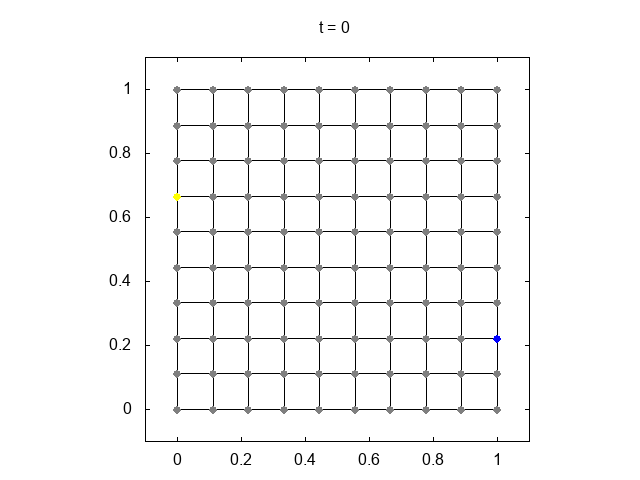
\includegraphics[width=1\textwidth]{t000}
    \centering
    \caption{Ejemplo de grafo dispuesto en forma de red con $10^2$ nodos colocados de diez en diez y conectados con vecinos a una distancia Manhattan de uno. En azul se muestra el nodo inicial $s$ y en amarillo el nodo final $t$.}
    \label{t000}
  \end{figure}

  En esta práctica se ha implementado un algoritmo de contracción de nodos que permita aproximar el flujo máximo que existe entre un nodo inicial $s$ y uno final $t$ calculado por el algoritmo de Ford-Fulkerson. Primeramente, se eligen al azar dos nodos destinados a ser el nodo inicial $s$ y el final $t$ del grafo. A partir de estos nodos se calcula el flujo máximo mediante el algoritmo de Ford-Fulkerson. Posteriormente, se procede a realizar las contracciones. Las contracciones de nodos consisten en la elección al azar de un nodo $n$; luego se toma uno de sus vecinos $v$ de manera aleatoria. Si ese vecino no es $s$ o $t$, $v$ es contraído por $n$, lo que quiere decir que los vecinos de $v$ pasan a ser vecinos de $n$ y que $v$ es eliminado. Cuando $n$ ya cuenta entre sus vecindades con alguno de los vecinos de $v$, los pesos de las aristas que constituyen sus vecindades se suman. Esta operación se repite hasta que se tienen únicamente a $s$ y a $t$ conectados entre sí mediante un arco cuyo peso es la suma de todos los pesos elegidos al azar durante el algoritmo. Un ejemplo de este proceso puede consultarse en una animación \texttt{gif} alojada en \url{https://goo.gl/akzeSD} y una serie de cuatro imágenes en la figura \ref{ejemplosGrafos} (p. \pageref{ejemplosGrafos}).

  \begin{figure}[h] %https://tex.stackexchange.com/questions/167770/forcing-figure-with-4-subfigures-to-span-over-twocolumns
    \centering
    \begin{subfigure}[b]{0.45\textwidth}
      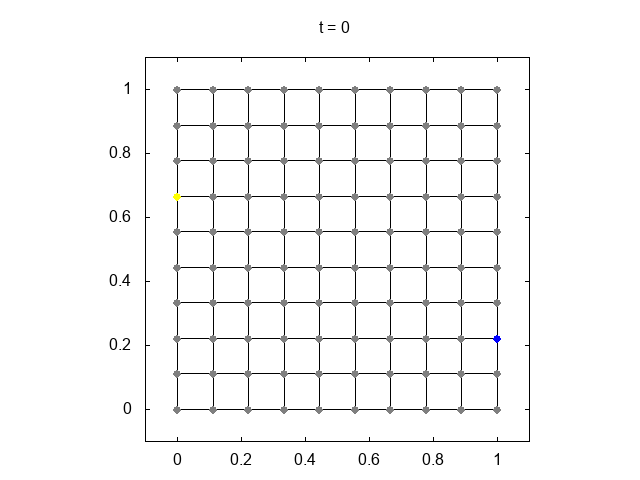
\includegraphics[width=\textwidth]{t000}
      \caption{Grafo inicial.}
      \label{fig:a}
    \end{subfigure}
    % this comment avoids break-line...
    \begin{subfigure}[b]{0.45\textwidth}
      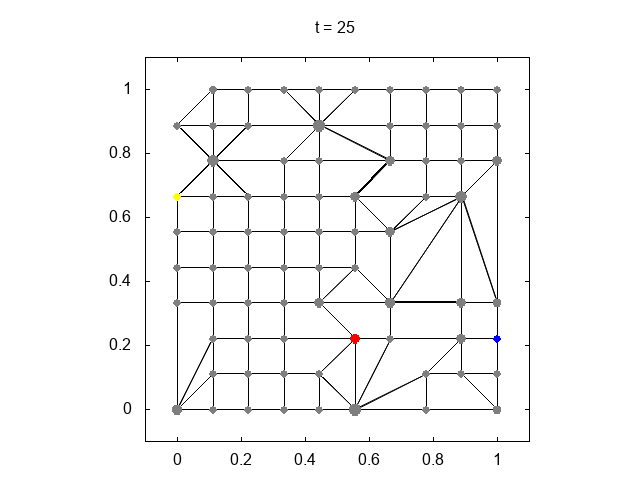
\includegraphics[width=\textwidth]{t025}
      \caption{Grafo en paso $25$.}
      \label{fig:b}
    \end{subfigure}

    \begin{subfigure}[b]{0.45\textwidth}
      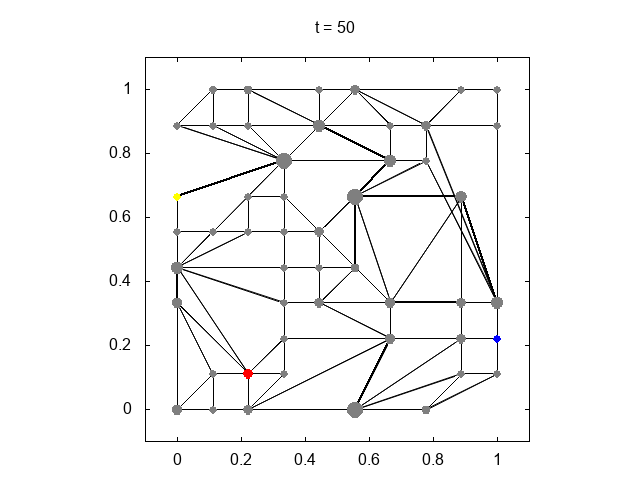
\includegraphics[width=\textwidth]{t050}
      \caption{Grafo en paso $50$.}
      \label{fig:c}
    \end{subfigure}
    % ... this comment too
    \begin{subfigure}[b]{0.45\textwidth}
      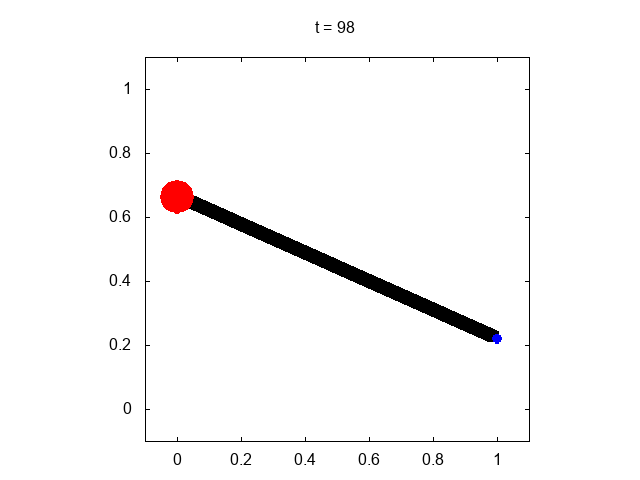
\includegraphics[width=\textwidth]{t098}
      \caption{Grafo final.}
          \label{fig:d}
    \end{subfigure}
    \caption{Muestra del avance de contracción en un grafo de $10^2$ nodos dispuestos en forma de red. El grosor de los arcos indica el peso del nodo, el nodo en azul es el nodo inicial $s$, el amarillo es el final $t$ y el rojo representa el nodo que en el paso mostrado fue contrajo a su vecino.}\label{ejemplosGrafos}
\end{figure}

  A continuación se corrieron instancias del algoritmo hasta que se lograra aproximar el flujo un $5$\% por encima del flujo calculado por el algoritmo de Floyd-Warshall y se graficaron los resultados en la figura \ref{flujo} (p. \pageref{flujo}).

  \begin{figure}[h]
    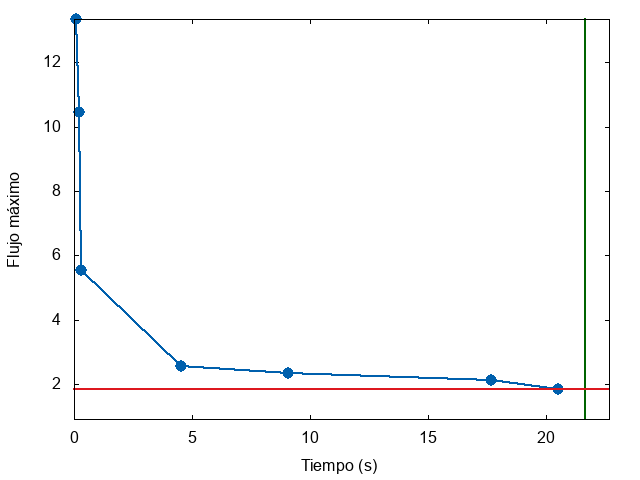
\includegraphics[width=1\textwidth]{flujo}
    \centering
    \caption{Gráfica del flujo máximo calculado por el tiempo en segundos de corrida del algoritmo diseñado para esta práctica (en azul). La línea horizontal roja representa el flujo máximo calculado por Floyd-Warshall y la línea vertical verde el tiempo que este último algoritmo tomó en ejecutarse.}
    \label{flujo}
  \end{figure}

  \bibliography{biblio}{}
  \bibliographystyle{plain}

\end{document}
